  Thus, the procedure is to calculate $\Hi{\chiFunc}_{\prd}$ at the points
  $\vctr{\mu}_{\prd}$ corresponding to the log of the $\aboveMin
  \vctr{m}_{\prd}$ points defined above, and then using these to construct an
  interpolating approximation $\Aprx{\Hi{\chiFunc}}_{\prd}$ from which we indirectly obtain our
  approximated consumption rule $\Aprx{\Hi{\cFunc}}_{\prd}$ by substituting $\Aprx{\Hi{\chiFunc}}_{\prd}$ for $\Hi{\chiFunc}$ in equation \eqref{eq:cFuncHi}.

  Because this method relies upon the fact that the problem is easy to
  solve if the decision maker has unreasonable views (either in the
  optimistic or the pessimistic direction), and because the correct
  solution is always between these immoderate extremes, we call our
  solution procedure the `method of moderation.'

  Results are shown in Figure~\ref{fig:ExtrapProblemSolved}; a reader
  with very good eyesight might be able to detect the barest hint of a
  discrepancy between the Truth and the Approximation at the far
  righthand edge of the figure\ctw{.}{ -- a stark contrast with the calamitous
    divergence evident in Figure~\ref{fig:ExtrapProblem}.}{}
  \hypertarget{ExtrapProblemSolvedPlot}{}
  \begin{figure}
    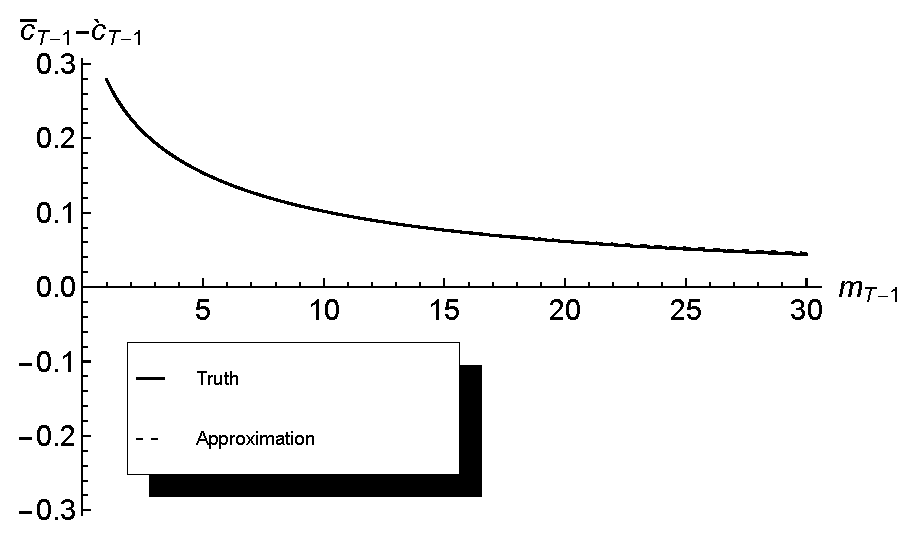
\includegraphics[width=6in]{./Figures/ExtrapProblemSolvedPlot}
    \caption{Extrapolated $\Aprx{\Hi{\cFunc}}_{\prd-1}$ Constructed Using the Method of Moderation}
    \label{fig:ExtrapProblemSolved}
  \end{figure}
